\documentclass{jreport}
\usepackage{xcolor}
\usepackage{amsmath}
\usepackage{amsfonts}
\usepackage{amssymb}
\usepackage{amsthm}
\usepackage{bm}
\usepackage{romannum}
\usepackage[dvipdfmx,hidelinks]{hyperref}
\usepackage{pxjahyper}
\usepackage{framed}
\usepackage{pifont}
\usepackage[dvipdfmx]{graphicx}
\begin{document}
\title{第四回レポート問題}
\author{習近平}
\setcounter{chapter}{4}
\maketitle
\newpage
\tableofcontents
\newpage
\section{問1}
5042
$A_m$を求めたいので,三角関数の直交性を用いて,式(1.1)の両辺に$\cos \left(n \pi \frac{x}{l} \right),n \in \mathbb{N}$をかけて,$0$から$l$まで積分すると次のような式が得られる:
\begin{equation}
	\begin{aligned}
		\int_0^l f(x) \cos \left( n \pi \frac{x}{l} \right) dx &=a \left( \int_0^{\frac{l}{2}} \cos\left(n \pi \frac{x}{l} \right) dx  - \int_{\frac{l}{2}}^l \cos\left(n \pi \frac{x}{l}\right) dx \right) \\
&= \frac{al}{n\pi} \left( \left[ \sin\left(n\pi \frac{x}{l} \right) \right]_0^{\frac{l}{2}} - \left[ \sin\left(n\pi \frac{x}{l} \right) \right]_{\frac{l}{2}}^l \right) \\
&= \frac{2al}{n \pi} \sin\left(\frac{n\pi}{2} \right)\\
&= A_n \frac{l}{2}
	\end{aligned}
\end{equation}
したがって,$A_m$の値は次のようになる:
$$
A_m = \frac{4a}{m\pi} \sin \left( \frac{m\pi}{2} \right)
$$
$ m=3,10,100 $ について $ f(x) $ をプロットした結果が以下のようなグラフとなる:
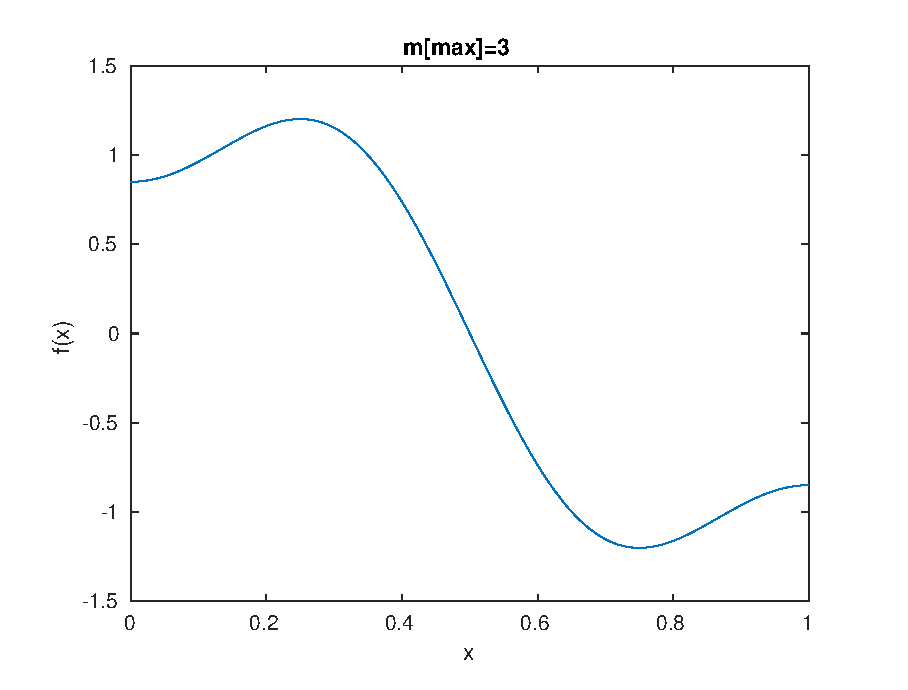
\includegraphics[scale=0.3]{1_3.eps}
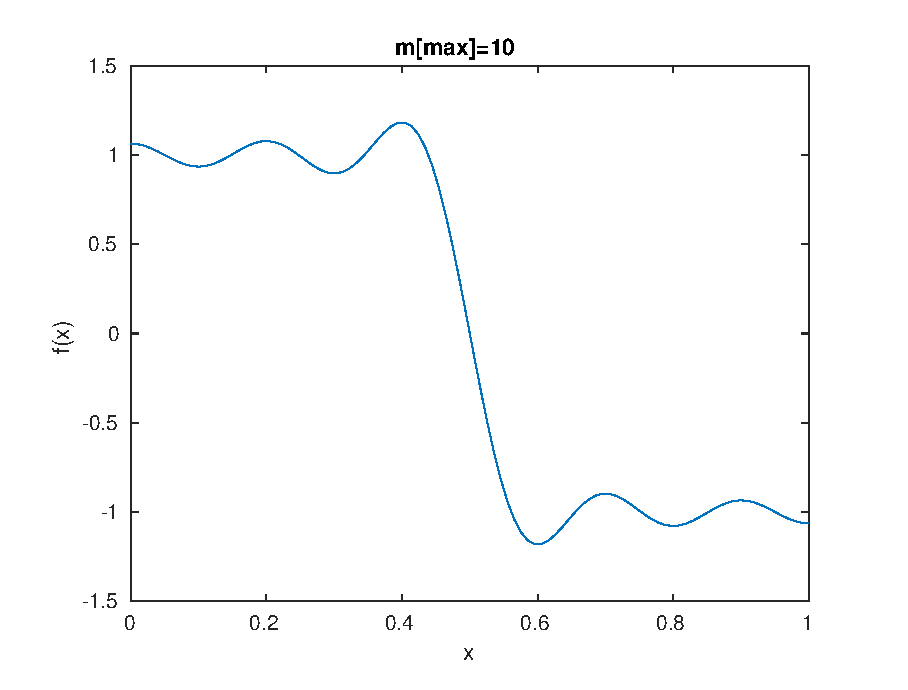
\includegraphics[scale=0.3]{1_10.eps}
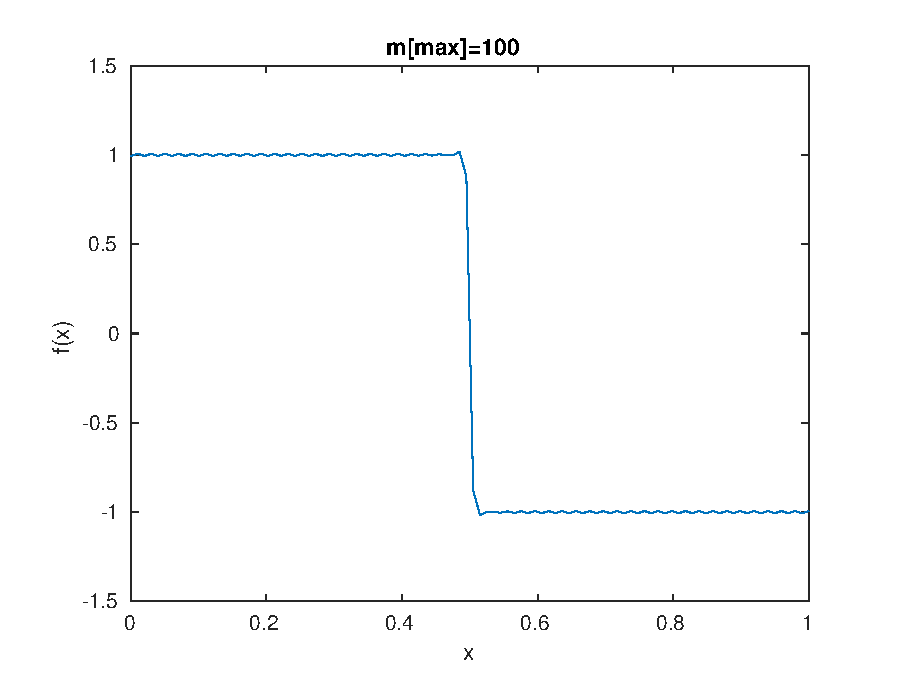
\includegraphics[scale=0.3]{1_100.eps}
\newpage
\section{問2}
時間変化のグラフは次のように与えられる.\\
\includegraphics[scale=0.3]{t0.eps}
\includegraphics[scale=0.3]{t25.eps}
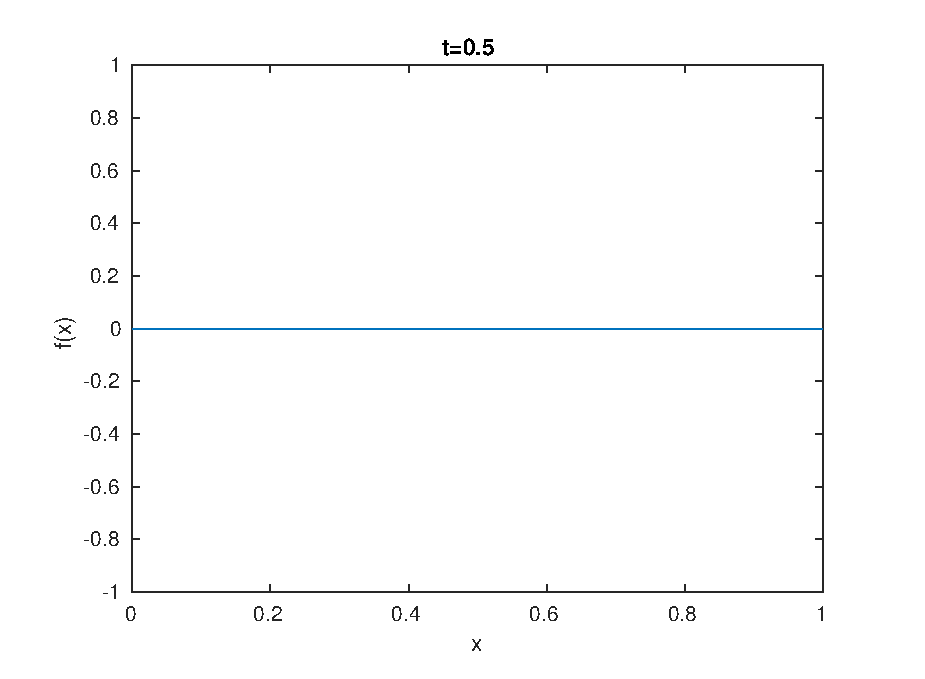
\includegraphics[scale=0.3]{t5.eps}
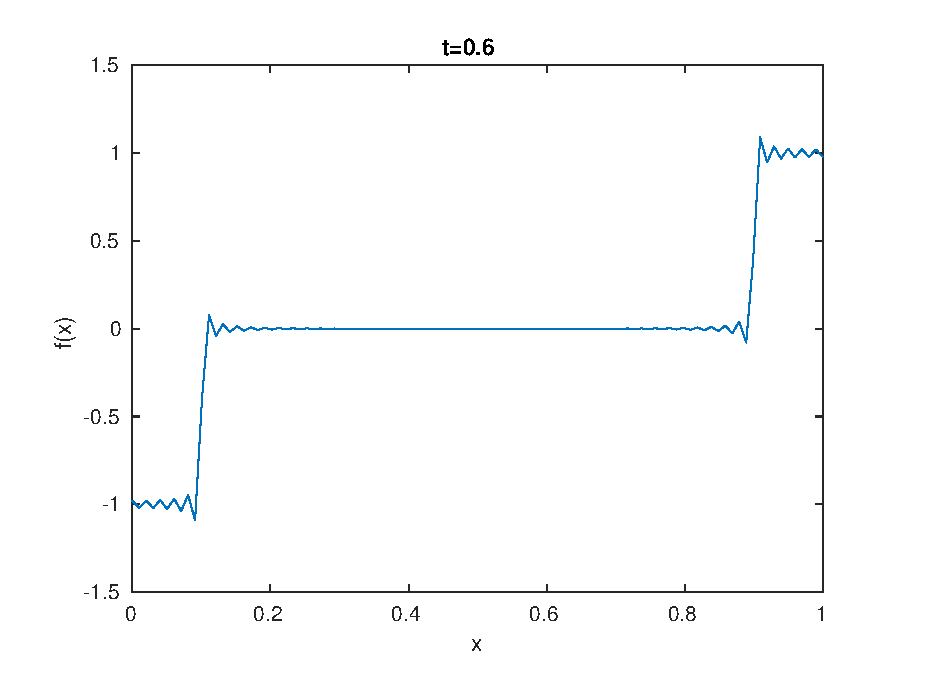
\includegraphics[scale=0.3]{t6.eps}
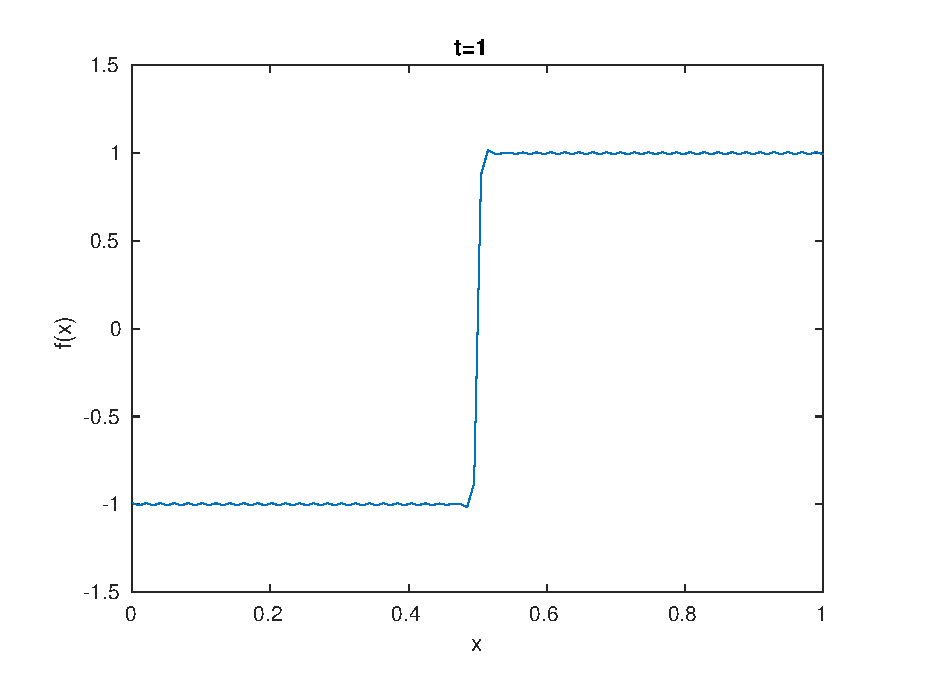
\includegraphics[scale=0.3]{t1.eps}\\
次にダランベル法で得られた時間変化のグラフは以下のように与えられる:\\
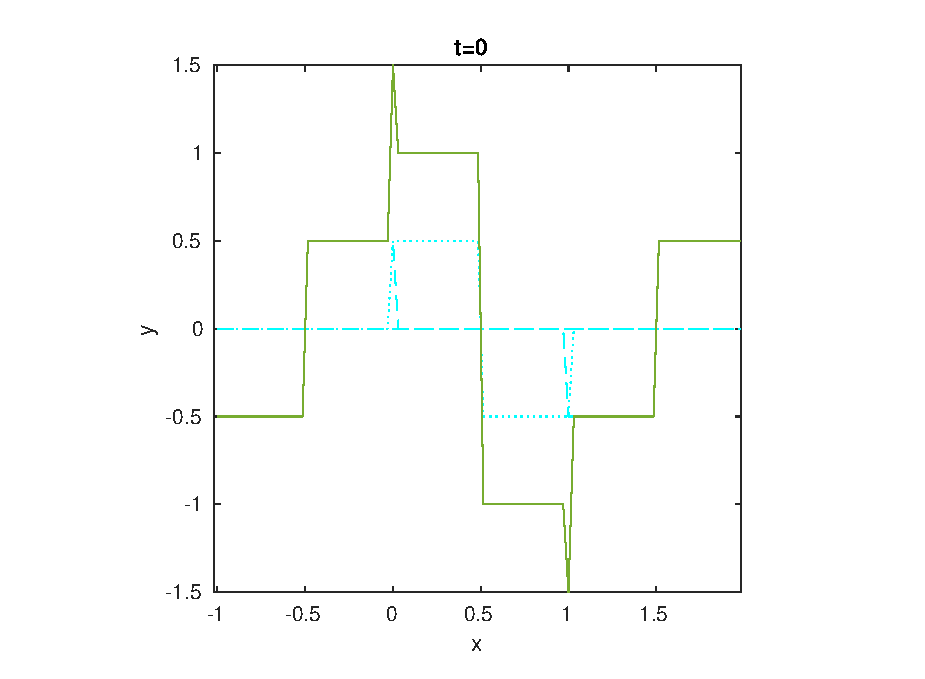
\includegraphics[scale=0.3]{20.eps}
\includegraphics[scale=0.3]{2125.eps}
\includegraphics[scale=0.3]{225.eps}
\includegraphics[scale=0.3]{2375.eps}
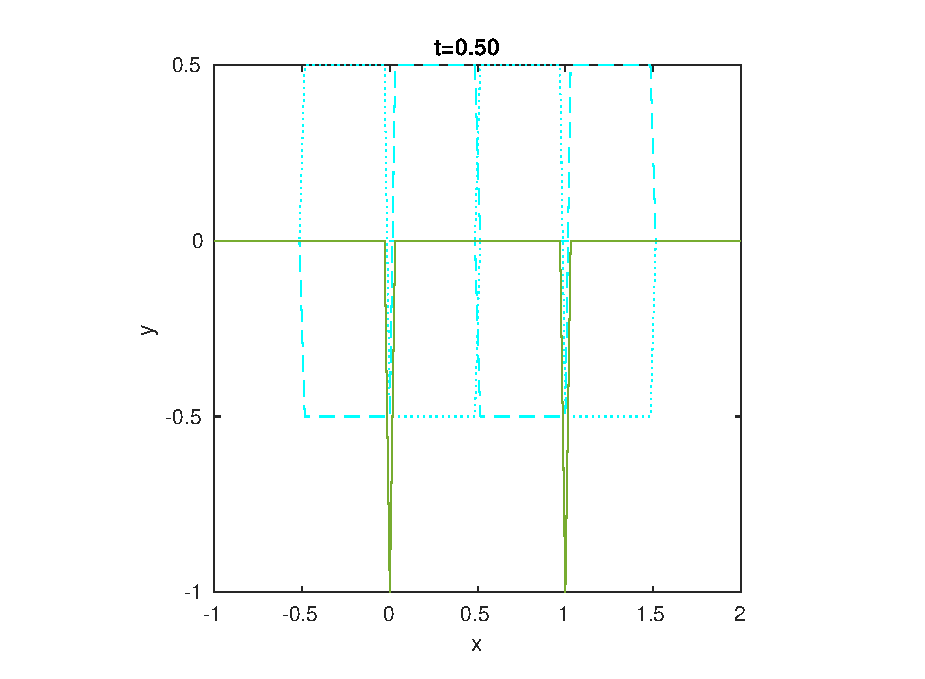
\includegraphics[scale=0.3]{250.eps}
\includegraphics[scale=0.3]{2625.eps}
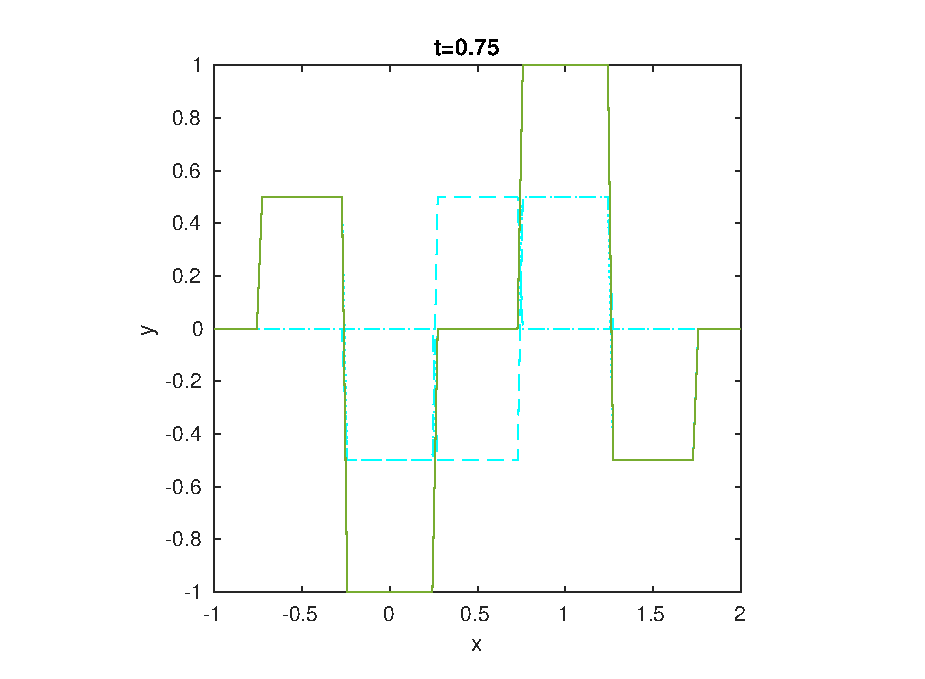
\includegraphics[scale=0.3]{275.eps}\\

緑の線は実際の合成波を表している.少し誤差が出ていますが閉区間$[0,1]$に着目すると同じ形で表されていることがわかる.
\end{document}


